% !TeX root = _main.tex
% ROLE 3: muc 7--9, giai phap, danh gia, thu nghiem va ket luan.
% Chi sua role cua minh va figures/rX_*. Khong sua tay bang do Python sinh.
% Nguoi ghep bai quan ly _main.tex va _content.tex.
% Macro Role*Supplement cuoi file giu ban nhap mo rong; KHONG duoc goi trong PDF.

\section{Phương án cải tiến và phân bổ nhân lực}
\label{r3:tobe}
\subsection{Từ hai nguyên nhân đến ba phương án}
Hai nguyên nhân đã chỉ ra ở Mục~\ref{r1:asis} và Mục~\ref{r2:diagnosis} dẫn
thẳng tới hai hướng cải tiến. Nguyên nhân thứ nhất là số kênh $c_t$ giữ cố
định trong khi lượng xe $\lambda_t$ thay đổi theo giờ. Nguyên nhân thứ hai là
thời gian phục vụ $E[S]$ dài vì việc trả tiền và lấy hóa đơn diễn ra ngay tại
trụ. Nhóm đưa mỗi hướng vào một phương án riêng để đo được tác động của từng
hướng (Bảng~\ref{r3:scenarios-design}).

\begin{table}[htbp]\centering\small
\caption{Ba phương án được so sánh trên cùng dòng xe đến mô phỏng}\label{r3:scenarios-design}
\begin{tabularx}{\linewidth}{@{}p{25mm}Y Y Y@{}}
\toprule
 & A0: AS-IS & A1: lịch theo giờ & A2: lịch theo giờ và trả trước \\
\midrule
Số kênh $c_t$ & 6 kênh ở mọi giờ & Theo BT1, dùng $E[S]$ hiện tại & Theo BT1, dùng $E[S]$ sau cải tiến \\
$E[S]$ (phút/xe) & Xe máy 1,5; ô tô 4,0 & Như A0 & Giảm 20\% (giả định): 1,2 và 3,2 \\
Thanh toán & Tiền mặt hoặc QR tại trụ & Như A0 & Trả trước trên ứng dụng; tiền mặt chỉ dùng khi lỗi \\
\bottomrule
\end{tabularx}
\end{table}

Cách đặt phương án như vậy giúp tách tác động theo từng bước. So A1 với A0
cho biết riêng việc xếp lịch theo giờ giúp được bao nhiêu, vì quy trình và
$E[S]$ giữ nguyên. So A2 với A1 cho biết rút ngắn thời gian phục vụ còn thêm
được gì. Tuy vậy, A2 đổi cả $E[S]$ lẫn lịch nên chưa tách được tác động riêng
của việc trả trước. Mức giảm 20\% cũng là giả định (G) trong
Bảng~\ref{r2:assumptions}, chưa có số đo.

\subsection{Lập lịch theo giờ (BT1)}
Lịch của A1 và A2 được lập bằng một bài toán, gọi tắt là BT1. Bài toán chọn
số kênh cho từng giờ sao cho chi phí nhân lực nhỏ nhất mà vẫn đạt mục tiêu về
thời gian chờ. Với chi phí $k=58\,000$ đồng cho một giờ nhân viên và 16 khung một
giờ từ 06:00 đến 22:00, bài toán được viết như sau:
\begin{align}
\min_{c_1,\ldots,c_{16}}\quad & k\textstyle\sum_{t=1}^{16}c_t \\
\text{với}\quad & c_t\in\{1,\ldots,8\},\ \rho_t<1,\ E[W_{q,t}]\le2\text{ phút},\ P(W_{q,t}>5)\le0{,}05. \nonumber
\end{align}
Ràng buộc đầu tiên giới hạn số kênh trong 8 vòi bơm. Ba ràng buộc còn lại
tính bằng M/M/c ở Mục~\ref{r2:method}: kênh không quá tải, chờ trung bình
không quá 2 phút và không quá 5\% số xe chờ trên 5 phút. Vì chi phí cộng
theo từng giờ và mỗi ràng buộc chỉ liên quan tới một giờ, lời giải là chọn
số kênh nhỏ nhất đạt yêu cầu ở từng giờ. Tỷ lệ bỏ đi không có trong công
thức M/M/c, nên được kiểm tra sau bằng mô phỏng (Mục~\ref{r3:evaluation}).

\resulttable{tab_shift_plan.tex}{Số kênh theo giờ của ba phương án (lời giải BT1)}{r3:staffing}

A1 không cần thêm người mà chỉ dời người sang giờ đông. Phương án này dùng
7 kênh ở ba giờ đông nhất (08--09, 17--18 và 18--19) và chỉ 4--5 kênh ở các
giờ vắng. Vì thế, lịch A1 cần 88 giờ nhân viên mỗi ngày thay vì 96. A2 chỉ
cần 72 giờ, vì khi $E[S]$ giảm 20\% thì mỗi kênh phục vụ được 47,8 xe mỗi
giờ thay vì 38,3 xe.

Thêm một kênh vào giờ đông có tác dụng rất lớn, vì hàng chờ tăng rất nhanh
khi $\rho$ gần 1. Tính bằng công thức M/M/c ở Mục~\ref{r2:method}, giờ 18--19 với 6
kênh có $\rho=0{,}98$ và thời gian chờ trung bình 12,2 phút. Với 7 kênh,
$\rho$ giảm còn 0,84 và thời gian chờ chỉ còn 0,8 phút.

BT1 mới chỉ cho biết số kênh cần ở mỗi giờ, chưa phải lịch làm việc. Để có lịch thật, cửa hàng còn phải ghép các giờ này
thành ca cho từng người, dài 4--8 giờ và có giờ nghỉ. Bước ghép ca
này chưa được tính trong báo cáo.

\subsection{Quy trình TO-BE và quy tắc vận hành}
Quy trình TO-BE của A2 giữ các bước chính của AS-IS nhưng đổi thứ tự trả
tiền (Hình~\ref{r3:bpmn}). Khách tạo đơn trên ứng dụng, chọn loại xăng và số
tiền trước khi vào trụ. Khi tới lượt, khách đưa mã đơn và xác nhận trả tiền.
Nhân viên chỉ bơm sau khi máy POS báo đã nhận tiền. Hóa đơn điện tử được gửi
thẳng về ứng dụng, nên xe không phải đứng chờ đếm tiền, thối tiền hay lấy
hóa đơn giấy. Khách không dùng ứng dụng vẫn đi theo luồng AS-IS ở
Hình~\ref{r1:bpmn}.

\begin{figure}[!htbp]\centering
\resizebox{\linewidth}{!}{%
\begin{tikzpicture}[
  mf/.style={{Circle[open,length=1.4mm]}-{Stealth[length=2.2mm,open]},dashed,thick,blue!50!black},
  mlab/.style={font=\scriptsize\itshape,fill=white,inner sep=1pt,text=blue!50!black},
  blab/.style={font=\scriptsize},
  gx/.style={diamond,draw,thick,fill=white,minimum width=9mm,minimum height=9mm,inner sep=0pt,font=\large},
  bbox/.style={draw,thick,fill=gray!12}]
\def\W{24.0}
% ---- Pool Khach hang ----
\draw[thick] (0,0) rectangle (\W,-2.4);
\draw[thick] (0.6,0) -- (0.6,-2.4);
\node[rotate=90,font=\scriptsize\bfseries] at (0.3,-1.2) {Khách hàng};
% ---- Pool Cua hang: 2 lan ----
\draw[thick] (0,-2.9) rectangle (\W,-8.3);
\draw[thick] (0.6,-2.9) -- (0.6,-8.3);
\draw (1.2,-2.9) -- (1.2,-8.3);
\draw (0.6,-5.6) -- (\W,-5.6);
\node[rotate=90,font=\scriptsize\bfseries] at (0.3,-5.6) {Cửa hàng xăng dầu};
\node[rotate=90,font=\scriptsize] at (0.9,-4.25) {Nhân viên bơm};
\node[rotate=90,font=\scriptsize] at (0.9,-6.95) {POS / HĐĐT};
% ---- Pool hop den ----
\draw[bbox] (0,-8.8) rectangle (17.0,-9.6);
\node[font=\scriptsize\bfseries] at (8.5,-9.2) {Ngân hàng / ví điện tử};
\draw[bbox] (17.5,-8.8) rectangle (\W,-9.6);
\node[font=\scriptsize\bfseries] at (20.75,-9.2) {Cơ quan thuế (hệ thống HĐĐT)};
% ---- Quy trinh khach hang ----
\node[ev] (cs) at (1.7,-1.5) {};
\node[blab,below=0mm of cs] {xe đến};
\node[task] (c1) at (3.75,-1.5) {Tạo đơn trên ứng dụng\\(loại xăng, số tiền)};
\node[gx] (cg) at (6.1,-1.5) {$\times$};
\node[blab,below=0.3mm of cg] {$\ge$20 xe chờ?};
\node[evend] (cb) at (7.4,-0.55) {};
\node[blab,anchor=west] at (7.7,-0.55) {bỏ đi; đơn chưa thu tiền tự hủy};
\node[task] (c2) at (9.0,-1.5) {Xếp hàng\\chờ tới lượt};
\node[task] (c3) at (11.7,-1.5) {Vào trụ,\\đưa mã đơn};
\node[task] (c4) at (14.6,-1.5) {Xác nhận trả tiền\\trên ứng dụng};
\node[task] (c5) at (21.6,-1.5) {Nhận hóa đơn trên\\ứng dụng, rời trụ};
\node[evend] (ce) at (23.45,-1.5) {};
\draw[flow] (cs) -- (c1);
\draw[flow] (c1) -- (cg);
\draw[flow] (cg.north) |- node[pos=0.3,left,blab]{có} (cb);
\draw[flow] (cg.east) -- node[above,blab]{không} (c2);
\draw[flow] (c2) -- (c3);
\draw[flow] (c3) -- (c4);
\draw[flow] (c4) -- (c5);
\draw[flow] (c5) -- (ce);
% ---- Lan nhan vien bom ----
\node[ev] (ss) at (7.7,-3.65) {};
\node[blab,below=0mm of ss] {trụ rảnh};
\node[task] (s1) at (10.0,-3.65) {Mời xe kế tiếp\\vào trụ};
\node[task] (s2) at (12.6,-3.65) {Quét mã đơn\\trên POS};
\node[task] (s3) at (17.4,-4.85) {Thu tại trụ như AS-IS\\(tiền mặt / QR)};
\node[task] (s4) at (19.9,-3.65) {Bơm đúng số tiền\\đã trả};
\draw[flow] (ss) -- (s1);
\draw[flow] (s1) -- (s2);
% ---- Lan POS / HDDT ----
\node[task] (p1) at (15.2,-7.0) {Chờ ngân hàng\\báo có};
\node[gx] (pg) at (17.4,-7.0) {$\times$};
\node[blab,anchor=north west] at ($(pg.south)+(0.05,-0.05)$) {Đã nhận tiền?};
\node[task] (p2) at (21.7,-7.0) {Xuất HĐĐT,\\gửi về ứng dụng};
\node[evend] (pe) at (23.45,-7.0) {};
\node[blab,anchor=south] at (pe.north) {xong};
\draw[flow] (s2.south) |- (p1.west);
\draw[flow] (p1) -- (pg);
\draw[flow] (pg.north) -- node[pos=0.45,left,blab,align=right]{không\\(lỗi, quá hạn)} (s3.south);
\draw[flow] (pg.east) -| node[pos=0.25,above,blab]{có} (s4.south);
\draw[flow] (s3.north) |- (s4.west);
\draw[flow] (s4.east) -| (p2.north);
\draw[flow] (p2) -- (pe);
% ---- Luong thong diep ----
\draw[mf] (10.85,-3.2) -- node[mlab]{lời mời} (10.85,-1.95);
\draw[mf] (12.3,-1.95) -- node[mlab]{mã đơn} (12.3,-3.2);
\draw[mf] (15.0,-1.95) -- node[mlab,pos=0.25]{xác nhận trả} (15.0,-6.55);
\draw[mf] (14.6,-7.45) -- node[mlab]{lệnh thu} (14.6,-8.8);
\draw[mf] (15.8,-8.8) -- node[mlab]{báo có} (15.8,-7.45);
\draw[mf] (22.5,-6.55) -- node[mlab,pos=0.6]{hóa đơn} (22.5,-1.95);
\draw[mf] (21.7,-7.45) -- node[mlab]{dữ liệu HĐ} (21.7,-8.8);
% ---- Moc do va ghi chu ----
\node[tmark] at (9.0,-2.15) {$a_i$: vào hàng};
\node[tmark] at (10.0,-4.35) {$b_i$: bắt đầu phục vụ};
\node[tmark] at (20.6,-2.15) {$d_i$: rời trụ};
\node[tmark,anchor=west,align=left] at (1.4,-3.55) {\textbf{A1:} số người đứng trụ theo\\lịch $c_t$ từng giờ (Bảng~\ref{r3:staffing})};
\node[tmark,anchor=west,align=left] at (1.4,-4.9) {\textbf{$S$ giảm (giả định 20\%):} không\\đếm tiền, thối tiền, giao hóa đơn giấy};
\node[tmark,anchor=west,align=left] at (1.4,-6.6) {\textbf{Ngoại lệ:} đã thu tiền mà không bơm\\được (vòi hỏng, hết xăng) thì hủy đơn,\\hoàn tiền; cuối ngày đối soát};
\end{tikzpicture}}
\caption{Quy trình TO-BE của A2: khách tạo đơn và trả tiền trước khi bơm, hóa đơn tự gửi về ứng dụng, số người đứng trụ theo lịch từng giờ. Ký pháp giống Hình~\ref{r1:bpmn}; khách không dùng ứng dụng vẫn đi theo luồng AS-IS.}
\label{r3:bpmn}
\source{nhóm vẽ bằng TikZ theo cùng ký pháp với hình AS-IS; Claude (Anthropic) hỗ trợ dựng mã hình; người viết role 3 kiểm tra ký pháp và luồng}
\end{figure}

Bảng~\ref{r3:changes} tóm tắt những gì thay đổi về vai trò, công nghệ và
chính sách phục vụ. Thay đổi lớn nhất về vai trò là khách tự làm phần đặt
yêu cầu và trả tiền, còn nhân viên chỉ tập trung vào việc bơm. Về chính sách,
số người đứng trụ không còn cố định mà đi theo lượng xe từng giờ.

\begin{table}[htbp]\centering\small
\caption{Những gì thay đổi từ AS-IS sang TO-BE}\label{r3:changes}
\begin{tabularx}{\linewidth}{@{}p{23mm}Y Y p{27mm}@{}}
\toprule
Thành phần & AS-IS & TO-BE & Người phụ trách \\
\midrule
Số người đứng trụ & 6 người ở mọi giờ & Theo lịch $c_t$ của BT1; lập lại khi lượng xe đổi rõ & Cửa hàng trưởng \\
Đặt yêu cầu & Khách nói loại xăng và số tiền tại trụ & Khách tạo đơn trên ứng dụng trước khi vào trụ & Khách \\
Thanh toán & Sau khi bơm, bằng tiền mặt hoặc QR & Trước khi bơm, qua ví hoặc ngân hàng; tiền mặt chỉ dùng khi lỗi & POS, nhân viên bơm \\
Hóa đơn & Nhân viên giao tại trụ & Tự gửi về ứng dụng & POS / HĐĐT \\
Xử lý lỗi & QR lỗi thì thu lại tiền mặt & Báo có lỗi thì thu như AS-IS; đã thu mà không bơm được thì hoàn tiền & Nhân viên; cửa hàng trưởng đối soát \\
\bottomrule
\end{tabularx}
\end{table}

Quy trình mới cần thêm vài quy tắc để không sinh lỗi mới. Đơn chỉ là đơn
nháp, chưa thu tiền cho tới khi xe vào trụ, nên khách bỏ hàng thì đơn tự hủy.
Hai tình huống lỗi còn lại được xử lý như ở dòng cuối Bảng~\ref{r3:changes}.
Cuối ngày, cửa hàng trưởng đối soát, tức là kiểm tra số tiền đã thu có khớp
với lượng xăng đã bơm hay không.

TO-BE cũng có những đánh đổi cần tính trước. Lợi ích của A2 phụ thuộc vào số
khách chịu dùng ứng dụng; nếu ít người dùng, $E[S]$ sẽ giảm ít hơn 20\%. Cửa
hàng phải trả chi phí ứng dụng và thanh toán, được giả định là 250 nghìn đồng
mỗi ngày, chưa kể chi phí đào tạo. Ngoài ra, cả A1 và A2 đều bớt người ở giờ
vắng, nên phần dự phòng khi có sự cố nhỏ hơn AS-IS (Mục~\ref{r3:scen3}).
\FloatBarrier

\section{Đánh giá, độ nhạy và giới hạn}
\label{r3:evaluation}
\subsection{So sánh trên cùng bộ chỉ số}
Bảng~\ref{r3:comparison} so sánh ba phương án trên cùng 20 ngày mô phỏng. Cả
ba phương án dùng chung một dòng xe đến, nên chênh lệch giữa các cột đến từ
phương án chứ không đến từ dữ liệu.

\resulttable{tab_comparison.tex}{Kết quả mô phỏng 20 ngày; ba phương án dùng chung dòng xe đến}{r3:comparison}

A1 giải quyết được vấn đề ở giờ cao điểm mà còn dùng ít giờ nhân viên hơn.
Trong khung 17--19, tỷ lệ xe chờ quá 5 phút giảm từ 6,18\% xuống 0,50\%, còn
tỷ lệ bỏ đi giảm từ 2,26\% xuống 0,17\%. Cả hai đều dưới ngưỡng 5\% và 1\%
đặt ra ở Mục~\ref{r1:scope}. Cùng lúc đó, lịch A1 cần ít hơn 8 giờ nhân viên mỗi
ngày, tương đương 464 nghìn đồng theo mô hình. Lý do là A1 chuyển người từ giờ vắng sang giờ
đông chứ không thêm người.

Cái giá của A1 là nhiều xe phải chờ một chút hơn ở giờ vắng. Tỷ lệ xe phải
chờ tăng từ 40,9\% lên 43,8\%, và mức sử dụng nhân viên tăng từ 67,9\% lên
74,5\%. Tuy vậy, các lần chờ này rất ngắn: 90\% số xe chờ không quá 1,51
phút, so với 2,37 phút ở A0. Như vậy, A1 đổi nhiều lần chờ rất ngắn để lấy
ít lần chờ dài.

A2 chủ yếu giúp tiết kiệm nhân lực chứ không giảm chờ thêm nhiều. Ở khung
17--19, thời gian chờ trung bình chỉ giảm từ 0,56 xuống 0,36 phút so với A1,
nhưng lịch A2 cần ít hơn 16 giờ nhân viên mỗi ngày. Sau khi trừ 250 nghìn đồng chi
phí công nghệ, A2 rẻ hơn A1 678 nghìn đồng và rẻ hơn A0 khoảng 1,14 triệu
đồng mỗi ngày. Đây chỉ là mức tiềm năng, vì nó dựa trên giả định $E[S]$ giảm
20\% và chưa tính chi phí chuyển đổi. Tính cả ngày, A2 còn có tỷ lệ chờ quá
5 phút (0,48\%) và lần chờ dài nhất (9,10 phút) cao hơn A1. Lý do là A2 ít
người hơn nên ít dư ra để đỡ những lúc xe dồn.

\subsection{Ba kịch bản: nhu cầu thấp, nhu cầu cao và thiếu người}
\label{r3:scen3}
Để xem các phương án có vững không, nhóm giữ nguyên lịch đã lập và thử ba
kịch bản. Hai kịch bản đầu đổi lượng xe đến: giảm 20\% (nhu cầu thấp) và tăng
20--40\% (nhu cầu cao). Kịch bản thứ ba là gián đoạn phục vụ do thiếu một
nhân viên. Mỗi cấu hình chạy 30 ngày với dòng xe đến khác
Bảng~\ref{r3:comparison}, nên mức cơ sở chênh nhẹ. Vì vậy chỉ nên so các
phương án trong cùng một bảng.

\resulttable{tab_sensitivity.tex}{Kết quả khi lượng xe đến thay đổi, giữ nguyên lịch (30 ngày mỗi cấu hình)}{r3:sensitivity}

Khi nhu cầu thấp, cả ba phương án đều đạt mục tiêu. Với lượng xe bằng 80\%
mức cơ sở, tỷ lệ chờ quá 5 phút của cả ba chỉ từ 0,01\% đến 0,12\%. Như vậy,
lịch theo giờ không gây hại khi vắng khách mà vẫn giữ được phần giờ công
tiết kiệm.

Khi nhu cầu cao, lịch đã lập nhanh chóng mất tác dụng. Với lượng xe tăng
20\%, A0 có 2,88\% khách bỏ đi, vượt ngưỡng 1\%. A1 vừa chạm ngưỡng với
0,95\%, vì giờ cao điểm đã có $\rho=1{,}01$. A2 còn dư hơn một chút với
0,53\%. Khi lượng xe tăng 40\%, cả ba đều không đạt, với 4,8--7,9\% khách bỏ
đi. Lúc này A1 thậm chí có tỷ lệ chờ quá 5 phút cao hơn A0 (14,81\% so với
10,83\%), vì A1 đã bớt người ở giờ vắng. Điều này cho thấy một lịch chỉ đúng
với mức nhu cầu dùng để lập nó, nên phải lập lại khi lượng xe thay đổi rõ.

\resulttable{tab_risk.tex}{Các tình huống rủi ro của A2 (30 ngày mỗi tình huống)}{r3:risks}

Thiếu người là rủi ro lớn nhất của các lịch đã bớt người. Khi A2 thiếu một nhân
viên ở mọi giờ, tỷ lệ chờ quá 5 phút tăng từ 0,48\% lên 16,71\% và 1,92\%
khách bỏ đi (Bảng~\ref{r3:risks}). Với A1, thiếu một người trong khung 17--19
sẽ đưa số kênh về 6, đúng như AS-IS. Theo Bảng~\ref{r2:hourly}, giờ 18--19
khi đó lại có $\rho=0{,}98$ và thời gian chờ trung bình khoảng 12 phút. Vì
vậy, cửa hàng cần một người dự phòng có thể gọi đến trong giờ cao điểm.

Rủi ro thứ hai của A2 là trả trước rút ngắn thời gian phục vụ ít hơn dự
kiến. Nếu chỉ giảm được 10\% thay vì 20\%, A2 vẫn đạt mục tiêu tính cả ngày,
với 1,45\% xe chờ quá 5 phút và 0,10\% khách bỏ đi. Tuy vậy, cần kiểm tra lại
từng giờ trước khi áp dụng.

\subsection{Độ nhạy theo các giả định chưa đo được}
Thời gian phục vụ, độ dao động của nó và ngưỡng bỏ đi đều là giả định (G)
trong Bảng~\ref{r2:assumptions}. Nhóm cho từng giả định lệch khỏi giá trị cơ
sở để xem kết luận có đổi không. Trong ba giả định này, $E[S]$ ảnh hưởng
mạnh nhất.

\resulttable{tab_sens_service.tex}{Kết quả khi $E[S]$ thực khác giả định ($\times$0,8--1,4), giữ nguyên lịch đã lập (30 ngày; $E[S]$ của A2 nhân cùng hệ số)}{r3:sens-service}

Nếu $E[S]$ thực dài hơn giả định mà lịch giữ nguyên, A1 sẽ không còn đạt mục
tiêu. Khi $E[S]$ dài hơn 20\% (xe máy 1,8 phút), A1 có 6,71\% xe chờ quá 5
phút và 1,00\% khách bỏ đi, dù vẫn tốt hơn A0 (11,53\% và 3,01\%). Khi dài
hơn 40\%, A1 còn kém A0 về tỷ lệ chờ quá 5 phút (38,58\% so với 29,34\%).
Ngược lại, nếu $E[S]$ ngắn hơn 20\%, cả ba phương án đều đạt.

\resulttable{tab_sens_replan.tex}{Giờ nhân viên cần nếu lập lại lịch theo $E[S]$ thực; ``không đạt'' là số giờ trong ngày không đạt mục tiêu dù mở đủ 8 vòi}{r3:sens-replan}

Nếu lập lại lịch theo $E[S]$ đo được, A1 vẫn dùng được nhưng sẽ chạm giới
hạn 8 vòi. Với $E[S]$ dài hơn 20\%, A1 cần 101 giờ nhân viên mỗi ngày thay vì
88, và vẫn có 1 giờ không đạt mục tiêu dù mở đủ 8 vòi. Với $E[S]$ dài hơn
40\%, A1 cần 114 giờ và có 3 giờ không đạt. Khi đó thêm người không còn giúp
được, vì đã hết vòi. A2 đạt mục tiêu ở mọi giờ trong cả bốn mức, kể cả mức
dài hơn 40\% (96 giờ nhân viên). Vì vậy, nếu $E[S]$ thực dài hơn giả định,
rút ngắn thời gian ở trụ trở thành điều kiện cần chứ không chỉ để tiết kiệm.

Hai giả định còn lại không làm đổi thứ tự giữa các phương án. CV là hệ số
biến thiên, bằng độ lệch chuẩn chia cho trung bình, cho biết thời gian phục
vụ dao động nhiều hay ít. Khi CV đi từ 0,5 đến 1,2, A1 luôn đạt mục tiêu, với
tỷ lệ chờ quá 5 phút không quá 0,84\%, và luôn tốt hơn A0. Ngưỡng bỏ đi chỉ
chuyển rủi ro qua lại giữa chờ lâu và mất khách. Với ngưỡng 10 xe, A0 mất
1,22\% khách; với ngưỡng 30 xe, A0 có 3,77\% xe chờ quá 5 phút. A1 đạt mục
tiêu ở cả hai trường hợp. Số liệu chi tiết nằm trong tệp
\texttt{tables/tab\_sens\_other.tex} của dự án.

Các kết quả độ nhạy cho thấy cách lập lịch theo $\lambda_t$ và $E[S]$ vẫn
đúng khi giả định lệch, nhưng số giờ công cụ thể phải tính lại từ $E[S]$ đo
thật. Do đó, việc bấm giờ thời gian phục vụ theo Phụ lục~\ref{r2:app-plan}
cần làm trước khi áp dụng lịch.

\subsection{Giới hạn}
Các kết quả trên đến từ mô hình nên còn bốn giới hạn chính. Lượt xe đến và
thời gian phục vụ là số mô phỏng; quy mô được hiệu chỉnh từ số liệu công bố
nhưng chưa đo tại cửa hàng nào. Mô hình coi mọi vòi phục vụ được mọi loại
xe, trong khi thực tế thường có trụ riêng cho ô tô. Ngưỡng bỏ đi 20 xe và mức
giảm 20\% thời gian phục vụ là giả định. Cuối cùng, mỗi ngày mô phỏng bắt đầu
với hàng rỗng, và ở tải rất cao kết quả mô phỏng lệch xa công thức
(Mục~\ref{r2:diagnosis}). Vì vậy, số liệu của giờ 18--19 chỉ nên xem là ước
lượng.

\section{Đề xuất triển khai và kết luận}
\label{r3:conclusion}
\subsection{Áp dụng lịch theo giờ trước, thử trả trước sau}
Nhóm đề xuất áp dụng A1 trước và chỉ thử A2 khi đã có số đo. Theo quy tắc
chọn ở Mục~\ref{r1:scope}, phương án được chọn phải đạt các ngưỡng, có chi
phí hợp lý và xếp được thành ca. A1 đạt các ngưỡng ở cả ngày lẫn giờ cao điểm,
rẻ hơn AS-IS và không cần thêm công nghệ. Riêng điều kiện xếp được thành ca
chưa được kiểm tra, nên đây là việc đầu tiên khi thử lịch (Bảng~\ref{r3:pilot}). A2 rẻ hơn nữa trong mô hình, nhưng lợi ích
dựa trên mức giảm 20\% chưa đo được, cần khách dùng ứng dụng và có ít dự
phòng khi thiếu người.

Khi áp dụng A1, cửa hàng cần thêm hai quy tắc vận hành. Thứ nhất, luôn có
một người dự phòng có thể gọi đến trong khung 17--19, vì thiếu một người ở
giờ này đưa cửa hàng về đúng tình trạng AS-IS. Thứ hai, lịch phải được lập
lại khi lượng xe giờ đông tăng gần 20\%, là mức mà lịch A1 vừa chạm ngưỡng
bỏ đi (Mục~\ref{r3:scen3}). Bảng~\ref{r3:pilot} nêu các bước thử trước khi
áp dụng rộng.

\begin{table}[htbp]\centering\small
\caption{Kế hoạch kiểm tra giải pháp trước khi áp dụng rộng}\label{r3:pilot}
\begin{tabularx}{\linewidth}{@{}p{24mm}Y Y@{}}
\toprule
Bước & Việc cần làm và người phụ trách & Tiêu chí quyết định \\
\midrule
Đo hiện trạng & Cửa hàng trưởng tổ chức ghi lượt đến, lượt bỏ đi và các mốc $a_i,b_i,d_i$ theo giờ; bấm giờ 30--50 lượt cho mỗi loại xe. Hóa đơn điện tử chỉ cho số lượt bán theo giờ, không cho giờ xe đến hay lượt bỏ đi. & Có số liệu cả giờ vắng và giờ đông; tách được thời gian bơm và thời gian trả tiền. \\
Thử lịch A1 & Ghép số kênh theo giờ thành ca có giờ nghỉ; thử trên các ngày cùng thứ, có lượng xe tương đương. & Tỷ lệ chờ quá 5 phút và tỷ lệ bỏ đi giờ đông giảm; ghi lại giờ công và chi phí thực. \\
Thử A2 ở phạm vi nhỏ & Cho một nhóm khách tạo đơn và trả trước; vẫn giữ cách trả tiền tại trụ. & Thời gian từ lúc vào trụ đến lúc rời trụ giảm; lỗi giao dịch không tăng; lợi ích đủ bù chi phí. \\
Rà soát định kỳ & Cửa hàng trưởng theo dõi số liệu theo giờ, ghi nhận nhu cầu tăng, người vắng và vòi hỏng. & Nếu vượt ngưỡng thì gọi người dự phòng hoặc lập lại lịch; không cố giữ mức tiết kiệm đã định. \\
\bottomrule
\end{tabularx}
\end{table}

\subsection{Kết luận}
Câu trả lời cho câu hỏi chính ở Mục~\ref{r1:scope} là có, trong phạm vi mô
hình. Chỉ cần xếp số nhân viên theo giờ (A1), tỷ lệ xe chờ quá 5 phút trong
khung 17--19 giảm từ 6,18\% xuống 0,50\% và tỷ lệ bỏ đi từ 2,26\% xuống
0,17\%, đều dưới ngưỡng. Trong khi đó, lịch tính toán chỉ cần 88 thay vì 96
giờ nhân viên mỗi ngày, dù con số này còn phải ghép thành ca và thử tại cửa
hàng. Cải tiến khâu thanh toán (A2) không cần để đạt ngưỡng ở kịch bản
cơ sở. Nó chủ yếu giúp tiết kiệm thêm nhân lực, và trở thành điều kiện cần
nếu thời gian phục vụ thực dài hơn giả định.

Đây là đề xuất dựa trên mô hình, chưa được kiểm chứng tại cửa hàng. Bước
tiếp theo là bấm giờ thời gian phục vụ, thử A1 trong một số ngày và chỉ mở
rộng khi các ngưỡng vẫn đạt; trả trước chỉ nên đầu tư khi đo được lợi ích.
\todo{3}{Chốt lịch ca khả thi, chi phí thực và kết quả thử nghiệm với cửa hàng;
không trình bày kết quả mô phỏng như thành tích đã triển khai.}

\newcommand{\RoleThreeSupplement}{%
\section{Kịch bản chiến lược và trải nghiệm khách hàng}
\label{r3:scenarios}
\subsection{Ba kịch bản tương lai và hai lựa chọn chiến lược}
Từ PESTEL (Bảng~\ref{r1:pestel}), nhóm xây ba kịch bản cho cửa hàng ở tầm
12--24 tháng. Xác suất chỉ dùng để tính chi phí kỳ vọng; tiêu chí chính là
hối tiếc tối đa, không phụ thuộc xác suất.
\begin{itemize}
\item \textbf{KB-A -- Nhu cầu thấp} (0,30): lượt xe $\times0{,}8$ do vùng phát
thải thấp mở rộng và khách chuyển sang xe điện~\cite{ct20,lez2026}.
\item \textbf{KB-B -- Nhu cầu tăng} (0,45): lượt xe $\times1{,}2$ do cửa hàng lân
cận đóng cửa vì chiết khấu thấp~\cite{chietkhau} và xe máy mới tăng~\cite{reg2025}.
\item \textbf{KB-C -- Gián đoạn} (0,25): như đợt tháng 3/2026~\cite{vtc2026},
khách dồn sang ($\times1{,}35$) và bán có kiểm soát làm thời gian phục vụ tăng 15\%.
\end{itemize}
Lựa chọn \textbf{CL-A -- nhân lực theo lịch, không số hóa} giữ lịch A1 (88 giờ).
Lựa chọn \textbf{CL-B -- số hóa} có hai biến thể: \emph{tĩnh} giữ lịch A2 (72 giờ);
\emph{thích ứng} dùng dự báo (Mục~\ref{r2:forecast}) để tối ưu lại $c_t$ theo
BT1 mỗi ngày, phần giờ vượt lịch A2 do nhân viên bán thời gian đảm nhận với đơn
giá $1{,}5\times58\,000$ đồng/giờ. Mỗi ô mô phỏng 30 ngày, cùng seed trong một
kịch bản.

\subsection{Mô hình mất khách theo thế hệ}
\label{r3:cx}
Mục tiêu dài hạn của chiến lược là khách quay lại, không bỏ cửa hàng. Một khách
thuộc phân khúc $g$ đã chờ $w$ phút có xác suất không hài lòng đến mức lần sau
bỏ đi là
\begin{equation}
p_g(w)=1-\exp\!\left[-(w/\theta_g)^2\right],
\end{equation}
dạng Weibull để chờ ngắn gần như không gây mất khách còn chờ dài làm xác suất
tăng nhanh; khách bỏ đi vì hàng dài có $p=1$. Mỗi lượt mất gây thiệt hại
$p\times[\text{lãi gộp lượt đó}+c_g\times\text{CLV}]$, với $c_g$ là xác suất
chuyển hẳn sang cửa hàng khác. CLV là lãi gộp 3 năm của một khách quen: xe máy
$73\times2{,}5\times1\,500\times3\approx820$ nghìn đồng, ô tô
$52\times30\times1\,500\times3\approx7{,}02$ triệu đồng. Các giá trị $\theta_g$,
$c_g$ trong Bảng~\ref{r3:segments} là giả định để thể hiện cơ chế, chưa có khảo sát.
\exttable{tab_ext_segments.tex}{Tỷ lệ mất khách theo phân khúc trong KB-B; $\theta_g$, $c_g$ là giả định}{r3:segments}
\textbf{Nhận định.} Với cùng một hàng chờ, Gen Z mất 8,79\% ở A0 so với 4,77\%
ở nhóm 60+. Khi chờ đã ngắn (CL-B thích ứng), khoảng cách tương đối còn lớn
hơn (1,41\% so với 0,50\%, gấp 2,8 lần): nhóm trẻ --- nhiều người là sinh viên
và tài xế giao hàng --- là nhóm đầu tiên rời đi và cũng là nhóm chuyển sang xe
điện sớm nhất. Hàm ý: thông báo thời gian chờ dự kiến và trả trước trên ứng
dụng cho nhóm trẻ; giữ thu tiền mặt và nhân viên hỗ trợ cho nhóm lớn tuổi.

\subsection{Kết quả theo kịch bản}
\exttable{tab_ext_scenarios.tex}{Hiệu quả của các chiến lược trong ba kịch bản; chi phí và giá trị mất tính bằng nghìn đồng/ngày}{r3:scen-table}
\begin{figure}[htbp]\centering
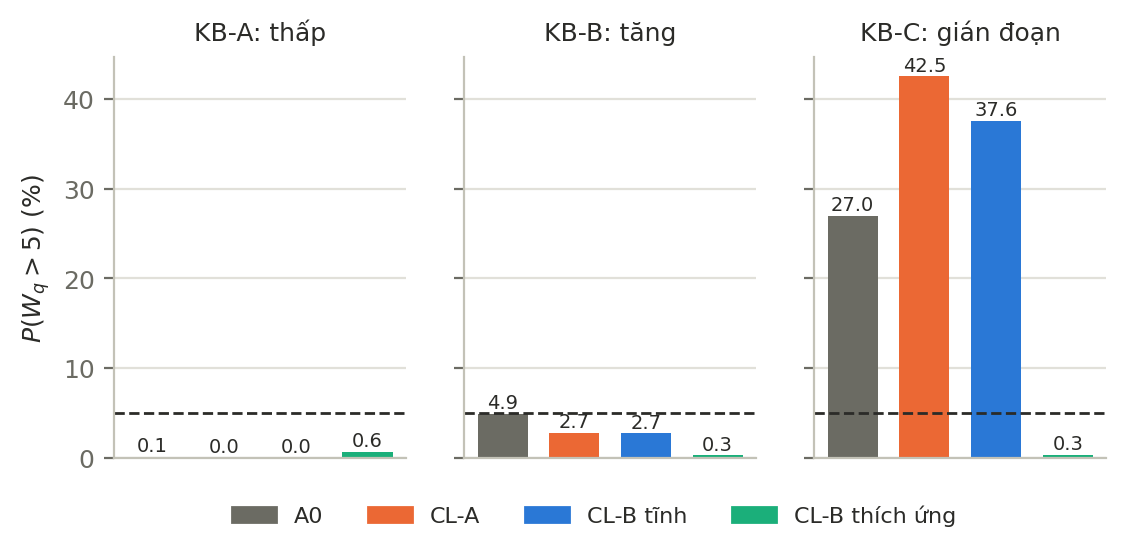
\includegraphics[width=0.92\linewidth]{figures/r3_scenarios.png}
\caption{Tỷ lệ xe chờ quá 5 phút theo kịch bản; đường đứt là mục tiêu 5\%.}
\label{r3:scen-fig}
\source{\texttt{analysis/extension\_analysis.py}; dữ liệu mô phỏng}
\end{figure}
(1) Ở KB-A mọi lựa chọn đều đạt; CL-B tĩnh rẻ nhất (4,68 triệu đồng/ngày) vì
biến thể thích ứng cắt xuống 59 giờ và làm chờ tăng nhẹ. (2) Ở KB-B, lịch tĩnh
vẫn đạt $P(W_q{>}5)\le5\%$ nhưng 3,6--4,4\% khách bị mất; CL-B thích ứng tăng lên
81 giờ và chỉ mất 0,98\%. (3) KB-C quyết định lựa chọn: mọi lịch tĩnh đều sụp
(37,6--42,5\% xe chờ quá 5 phút, 11,8--13,6\% bỏ đi), trong khi CL-B thích ứng
giữ 0,30\% với 101 giờ/ngày --- gần chạm giới hạn 8 vòi ở giờ cao điểm.
\exttable{tab_ext_regret.tex}{Tổng chi phí (nghìn đồng/ngày), kỳ vọng và hối tiếc tối đa; ``đạt'' khi $P(W_q{>}5)\le5\%$ và bỏ đi $\le1\%$}{r3:regret}

\subsection{Đánh giá và quyết định}
Nhóm chọn \textbf{CL-B thích ứng}: hối tiếc tối đa chỉ 554,8 nghìn đồng/ngày
(ở KB-A) so với 59--66 triệu đồng/ngày của hai lựa chọn tĩnh (ở KB-C); chi phí kỳ
vọng 7,31 so với 23,90--26,72 triệu đồng/ngày; và là lựa chọn duy nhất đạt mục
tiêu ở cả ba kịch bản.
\exttable{tab_ext_clv.tex}{Chi phí kỳ vọng (nghìn đồng/ngày) theo hệ số CLV}{r3:clv}
\textbf{Kết luận có bền không?} Ngay cả khi bỏ hoàn toàn giá trị khách quay lại
(CLV = 0, chỉ tính lãi gộp của lượt bị mất), CL-B thích ứng vẫn rẻ nhất
(5,34 so với 5,87 và 6,71 triệu đồng/ngày) vì khách bỏ đi trong KB-C là doanh
thu mất ngay. Điều kiện để kết luận đúng là \emph{dự báo đủ tốt} và \emph{có
nguồn nhân viên bán thời gian huy động được trong ngày}.

\subsection{Năng lực thích ứng nhờ dự báo}
\label{r3:ml-staff}
Mô hình GLM ở Mục~\ref{r2:forecast} được dùng để lập lịch $c_t$ cho từng ngày
kiểm tra; mỗi ngày được mô phỏng với nhu cầu thật của ngày đó.
\exttable{tab_ext_ml_staff.tex}{Lập lịch theo dự báo trên 84 ngày kiểm tra (5/1--29/3/2026); ngày vi phạm: $P(W_q{>}5)>5\%$ hoặc bỏ đi $>1\%$}{r3:ml-staff-table}
Lịch A2 tĩnh vi phạm ở 16,7\% số ngày và 10,67\% xe chờ quá 5 phút trong các
ngày sự kiện. Lịch theo GLM giảm số ngày vi phạm xuống 6,0\% mà chỉ dùng 70,48
giờ/ngày --- ít hơn lịch tĩnh. Phương án ``đệm 20\%'' đạt kết quả tương đương
(7,1\% ngày vi phạm) nhưng tốn 81 giờ/ngày; GLM tiết kiệm 10,5 giờ, tức 610
nghìn đồng/ngày (khoảng 18 triệu đồng/tháng). Lịch theo trung bình 4 tuần còn
kém lịch tĩnh (27,4\% ngày vi phạm) vì phản ứng trễ với sự kiện.

\begin{table}[htbp]\centering\small
\caption{Kế hoạch ứng phó: dấu hiệu sớm, ngưỡng kích hoạt và hành động}\label{r3:playbook}
\begin{tabularx}{\linewidth}{@{}p{14mm}Y Y Y@{}}
\toprule
Kịch bản & Dấu hiệu sớm & Ngưỡng kích hoạt & Hành động \\
\midrule
KB-A & Lượt xe dự báo giảm; vùng phát thải thấp mở rộng & $<2\,000$ lượt/ngày trong 4 tuần & Giảm kênh lúc vắng; đàm phán lắp tủ đổi pin/trạm sạc~\cite{vgx} \\
KB-B & Cửa hàng lân cận đóng cửa; dự báo tăng & $>2\,900$ lượt/ngày hoặc $\rho_{17-19}>0{,}85$ & Tối ưu lại $c_t$ ($\approx$81 giờ/ngày); tuyển thêm nhân viên bán thời gian \\
KB-C & Tin căng thẳng nguồn cung; điều chỉnh giá lớn & Tín hiệu nguồn cung hoặc $|\Delta p|\ge1\,000$ đồng/lít & Mở đủ 8 vòi giờ cao điểm; gọi ca dự phòng; hiển thị ETA, ưu tiên khách trả trước \\
\bottomrule
\end{tabularx}
\end{table}

\begin{table}[htbp]\centering\small
\caption{Học máy trong dịch vụ: tác động, chỉ số chấp nhận và kiểm soát}\label{r3:ml-uses}
\begin{tabularx}{\linewidth}{@{}p{27mm}Y Y Y@{}}
\toprule
Ứng dụng & Tác động lên mô hình & Chỉ số chấp nhận & Kiểm soát \\
\midrule
Dự báo lượt xe (đã thử) & $\hat\lambda_{d,h}\to c_t$ & MAPE $\le10\%$; ngày vi phạm $\le7\%$ & Cửa hàng trưởng duyệt lịch hằng ngày \\
Ước lượng độ kiên nhẫn & $\theta_g$ từ tỷ lệ bỏ đi theo độ dài hàng & Sai số dự báo bỏ đi & Chỉ dùng dữ liệu ẩn danh, gộp \\
Dự báo rời bỏ & Khách quen giảm tần suất & AUC; tỷ lệ giữ chân & Ưu đãi có đồng ý của khách \\
Phát hiện bất thường & Lượt bán đột biến, lỗi cột bơm & Thời gian phát hiện & Kiểm tra thủ công trước khi xử lý \\
\bottomrule
\end{tabularx}
\end{table}


}
